\documentclass[11pt,landscape]{article}
\usepackage{multicol}
\usepackage{calc}
\usepackage{ifthen}
\usepackage[landscape]{geometry}
\usepackage{hyperref}
\usepackage{amsmath}
\usepackage{graphicx}
\usepackage{float}

% To make this come out properly in landscape mode, do one of the following
% 1.
%  pdflatex latexsheet.tex
%
% 2.
%  latex latexsheet.tex
%  dvips -P pdf  -t landscape latexsheet.dvi
%  ps2pdf latexsheet.ps


% If you're reading this, be prepared for confusion.  Making this was
% a learning experience for me, and it shows.  Much of the placement
% was hacked in; if you make it better, let me know...


% To Do:
% \listoffigures \listoftables
% \setcounter{secnumdepth}{0}


% This sets page margins to .5 inch if using letter paper, and to 1cm
% if using A4 paper. (This probably isn't strictly necessary.)
% If using another size paper, use default 1cm margins.
\ifthenelse{\lengthtest { \paperwidth = 11in}}
	{ \geometry{top=.5in,left=.5in,right=.5in,bottom=.5in} }
	{\ifthenelse{ \lengthtest{ \paperwidth = 297mm}}
		{\geometry{top=1cm,left=1cm,right=1cm,bottom=1cm} }
		{\geometry{top=1cm,left=1cm,right=1cm,bottom=1cm} }
	}

% Turn off header and footer
\pagestyle{empty}
 

% Redefine section commands to use less space
\makeatletter
\renewcommand{\section}{\@startsection{section}{1}{0mm}%
                                {-1ex plus -.5ex minus -.2ex}%
                                {0.5ex plus .2ex}%x
                                {\normalfont\large\bfseries}}
\renewcommand{\subsection}{\@startsection{subsection}{2}{0mm}%
                                {-1explus -.5ex minus -.2ex}%
                                {0.5ex plus .2ex}%
                                {\normalfont\normalsize\bfseries}}
\renewcommand{\subsubsection}{\@startsection{subsubsection}{3}{0mm}%
                                {-1ex plus -.5ex minus -.2ex}%
                                {1ex plus .2ex}%
                                {\normalfont\small\bfseries}}
\makeatother

% Define BibTeX command
\def\BibTeX{{\rm B\kern-.05em{\sc i\kern-.025em b}\kern-.08em
    T\kern-.1667em\lower.7ex\hbox{E}\kern-.125emX}}

% Don't print section numbers
\setcounter{secnumdepth}{0}


\setlength{\parindent}{0pt}
\setlength{\parskip}{0pt plus 0.5ex}


% -----------------------------------------------------------------------

\begin{document}

\raggedright
\footnotesize
\begin{multicols}{3}


% multicol parameters
% These lengths are set only within the two main columns
%\setlength{\columnseprule}{0.25pt}
\setlength{\premulticols}{1pt}
\setlength{\postmulticols}{1pt}
\setlength{\multicolsep}{1pt}
\setlength{\columnsep}{2pt}

\begin{center}
     \Large{\textbf{EECS 301 Cheat Sheet}} \\
\end{center}

\section{Definitions}
$E[aX + b] = aE[X] + b$ \\
$\mathrm{Var}[X] = E[(x-\mu_X)^2] = \int_{-\infty}^{\infty} \! (x-\mu_X)^2f_X(x) \, \mathrm{d}x$ \\
$\mathrm{Var}[aX] = a^2\mathrm{Var}[X]$ \\
$\mathrm{Var}[X-b] = \mathrm{Var}[X]$ \\
Gaussian Distribution $F_X(x) = \Phi(\frac{x-\mu}{\sigma})$ \\
Gaussian Density $f_X(x) = \dfrac{1}{\sigma\sqrt{2\pi}}e^{\frac{-(x-\mu)^2}{2\sigma^2}}$ \\
$\Phi(x) = \int_{-\infty}^x \! \dfrac{1}{2\pi}e^{-t^2/2} \, \mathrm{d}t$
\hspace{10pt} $Q(x) = 1-\Phi(x) = \Phi(-x)$ \\
$E[X^2] = \sigma^2 + \mu^2$ \\
$F_{X|A}(x) = P\{X\leq x|A\} = \frac{P\{(X\leq x) \cap A\}}{P(A)}$
$\mathrm{Covariance}(X, Y) = E[(X-E[X])(Y - E[Y])]$

\section{Huffman's Algo}
\begin{multicols}{2}
\setlength{\premulticols}{1pt}
\setlength{\postmulticols}{1pt}
\setlength{\multicolsep}{1pt}
\setlength{\columnsep}{2pt}
\begin{figure}[H]
    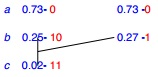
\includegraphics[scale=0.8]{./Images/2/Huffman.jpg}
\end{figure}
Entropy = \\ $-0.73log_2(0.73)$ \\$-0.25log_2(0.25)$ $-0.02log_2(0.02)$
\end{multicols}



\section{Continuous Random Variables}
Density Function $F_X(x) = P\{X\leq x\} = \int_{-\infty}^x \! f_x(u) \, \mathrm{d}u$ \\
Cumulative Dist Function $f_x(x) = \frac{\delta F_x(x)}{\delta x}$ \\
$\int_{-\infty}^{\infty} \! f_x(x) \, \mathrm{d}x = 1$ \hspace{10pt} $f_X(x) \geq 0$ \\
$E[X] = \int \! xf_X(x) \, \mathrm{d}x$

%---------------------------------------------------------------------------

\end{multicols}

\begin{multicols}{3}
\setlength{\premulticols}{1pt}
\setlength{\postmulticols}{1pt}
\setlength{\multicolsep}{1pt}
\setlength{\columnsep}{2pt}
\begin{figure}[H]
    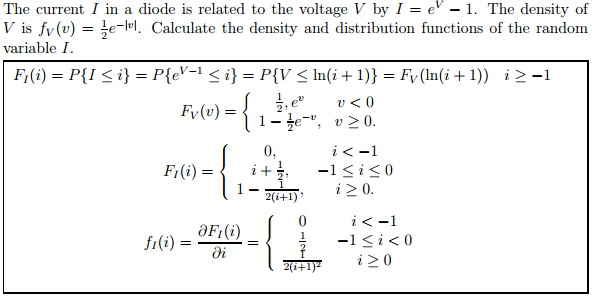
\includegraphics[scale=0.53]{./Images/2/DenDisSolve.jpg}
\end{figure}
\begin{figure}[H]
    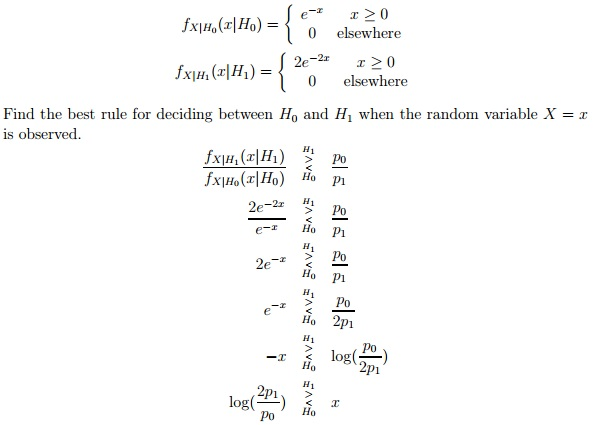
\includegraphics[scale=0.53]{./Images/2/Decision.jpg}
\end{figure}
\begin{figure}[H]
    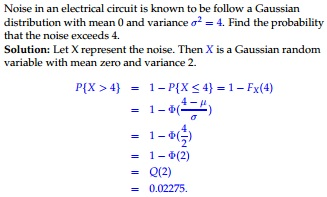
\includegraphics[scale=1]{./Images/2/qfunc.jpg}
\end{figure}
\begin{figure}[H]
    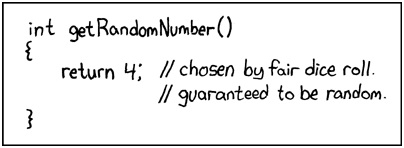
\includegraphics[scale=0.75]{./Images/1/RandNumXKCD.jpg}
\end{figure}
\end{multicols}

\end{document}
